\section{Metodología}
\label{sec:method}

\subsection{Planteamiento: comparación controlada de arquitecturas}

La contribución metodológica central de este trabajo es un \textbf{estudio
comparativo controlado de arquitecturas de red} para la inversión de
batimetría. Se evalúan tres familias de arquitectura sobre el mismo problema
inverso: la \textbf{propuesta de dos redes} de esta tesis (A1), una red
\textbf{monolítica} al estilo de Dazzi et al.\ \cite{dazzi2024} (A2), y una
arquitectura de \textbf{una red por campo} al estilo de Ohara et al.\
\cite{ohara2024} (A3). Para que la comparación sea justa y no quede sesgada por
la capacidad de cada red, cada diseño se evalúa mediante un \textbf{estudio de
escalamiento}: se instancia a un rango de presupuestos de parámetros, lo que
permite comparar los diseños a presupuesto igualado y, a la vez, trazar su
curva de precisión frente a costo. Todo se entrena bajo un protocolo de
comparación justa (Sección~\ref{sec:protocolo}) en el que el diseño de la
arquitectura es la única variable.

\subsection{Arquitecturas evaluadas}
\label{sec:arquitecturas}

Se comparan tres diseños de arquitectura (Tabla~\ref{tab:arch-cost}), cada uno
evaluado en un estudio de escalamiento sobre el mismo problema inverso.

\paragraph{A1 --- Propuesta: dos redes.}
La arquitectura propuesta separa el aprendizaje en dos redes neuronales:
\begin{itemize}
  \item \textbf{SolutionNet}: $(x, t) \to (h, u)$ --- campo de flujo, con
        embedding de Fourier \cite{tancik2020} ($\sigma = 2$, 16 frecuencias).
  \item \textbf{BathymetryNet}: $x \to \zb$ --- batimetría desconocida.
        \emph{No recibe $t$ como entrada}, lo que impone
        $\partial \zb/\partial t = 0$ estructuralmente.
\end{itemize}
La profundidad se fuerza no negativa por construcción,
$h = \softplus(\cdot)$, mientras que $\zb$ queda libre. En el presupuesto
pequeño la SolutionNet tiene 4 capas $\times$ 64 neuronas y la BathymetryNet
3 $\times$ 32 (17\,923 parámetros); el ancho y la profundidad se escalan para
los presupuestos mayores.

\paragraph{Embedding de Fourier.}
El embedding de Fourier \cite{tancik2020} mapea cada entrada $s$ a
$\gamma(s) = [\,\sin(2\pi \bm{B}s),\ \cos(2\pi \bm{B}s)\,]$, con
$\bm{B}\in\mathbb{R}^{m\times d}$ de entradas fijas
$B_{kj}\sim\mathcal{N}(0,\sigma^2)$ ($\sigma = 2$, $m = 16$ frecuencias). Esta
codificación mitiga el sesgo espectral de los PINN, que de otro modo aprenden
con lentitud las componentes de alta frecuencia de $\zb$. Es un rasgo
distintivo de A1: las arquitecturas A2 y A3 operan sobre las entradas crudas.

\paragraph{A2 --- Monolítica (estilo Dazzi).}
Imita la arquitectura de Dazzi et al.\ \cite{dazzi2024}
(Sección~\ref{sec:lit:dazzi}): una \emph{única} red MLP que recibe $(x,t)$ y
produce \emph{conjuntamente} $(h, u, \zb)$. La batimetría es
una salida más de la red; la condición $\partial\zb/\partial t = 0$ se impone
como término de pérdida y no estructuralmente. Opera sobre las entradas
crudas. Su escala nativa (7 capas $\times$ 300 neuronas, $\approx$544K
parámetros) corresponde al presupuesto grande del barrido.

\paragraph{A3 --- Una red por campo (estilo Ohara).}
Imita la arquitectura de Ohara et al.\ \cite{ohara2024}
(Sección~\ref{sec:lit:ohara}): una red totalmente conectada \emph{separada por
cada campo} de salida --- una para $h$, otra para $u$ (y otra para $v$ en 2D) y
otra para $\zb$ ---, en lugar de agrupar varios campos en una misma red. Opera
sobre las entradas crudas. Al igual que en A1, la red de $\zb$ no recibe $t$,
por lo que $\partial\zb/\partial t = 0$ se cumple de forma estructural. Su
escala nativa (8 capas $\times$ 60 neuronas por red) ronda los $\approx$100K
parámetros totales, el presupuesto medio del barrido.

\begin{table}[H]
\centering
\caption{Diseños de arquitectura comparados. Cada uno se evalúa en un estudio
         de escalamiento (presupuestos pequeño, medio y grande).}
\label{tab:arch-cost}
\begin{tabular}{@{}lccc@{}}
\toprule
Diseño & Redes & Encoding & $\partial\zb/\partial t = 0$ \\
\midrule
A1 Propuesta          & 2           & Fourier & estructural \\
A2 Monolítica (Dazzi) & 1           & crudo   & término de pérdida \\
A3 Por campo (Ohara)  & 1 por campo & crudo   & estructural \\
\bottomrule
\end{tabular}
\end{table}

\paragraph{Estudio de escalamiento.}
Cada diseño se instancia a tres presupuestos de parámetros --- pequeño
($\approx$20K), medio ($\approx$100K) y grande ($\approx$500K) --- ajustando
el ancho y la profundidad de las redes. Las tres escalas nativas abarcan los
tres presupuestos: A1 $\approx$18K (pequeño), A3 $\approx$100K (medio, una red
por campo estilo Ohara) y A2 $\approx$544K (grande, monolítica estilo Dazzi).
Comparar los tres diseños a presupuesto igualado
aísla el efecto del \emph{diseño} del de la \emph{capacidad}; barrer el
presupuesto traza la curva de precisión frente a número de parámetros de cada
diseño (Sección~\ref{sec:arch-comp}).

\begin{figure}[H]
  \centering
  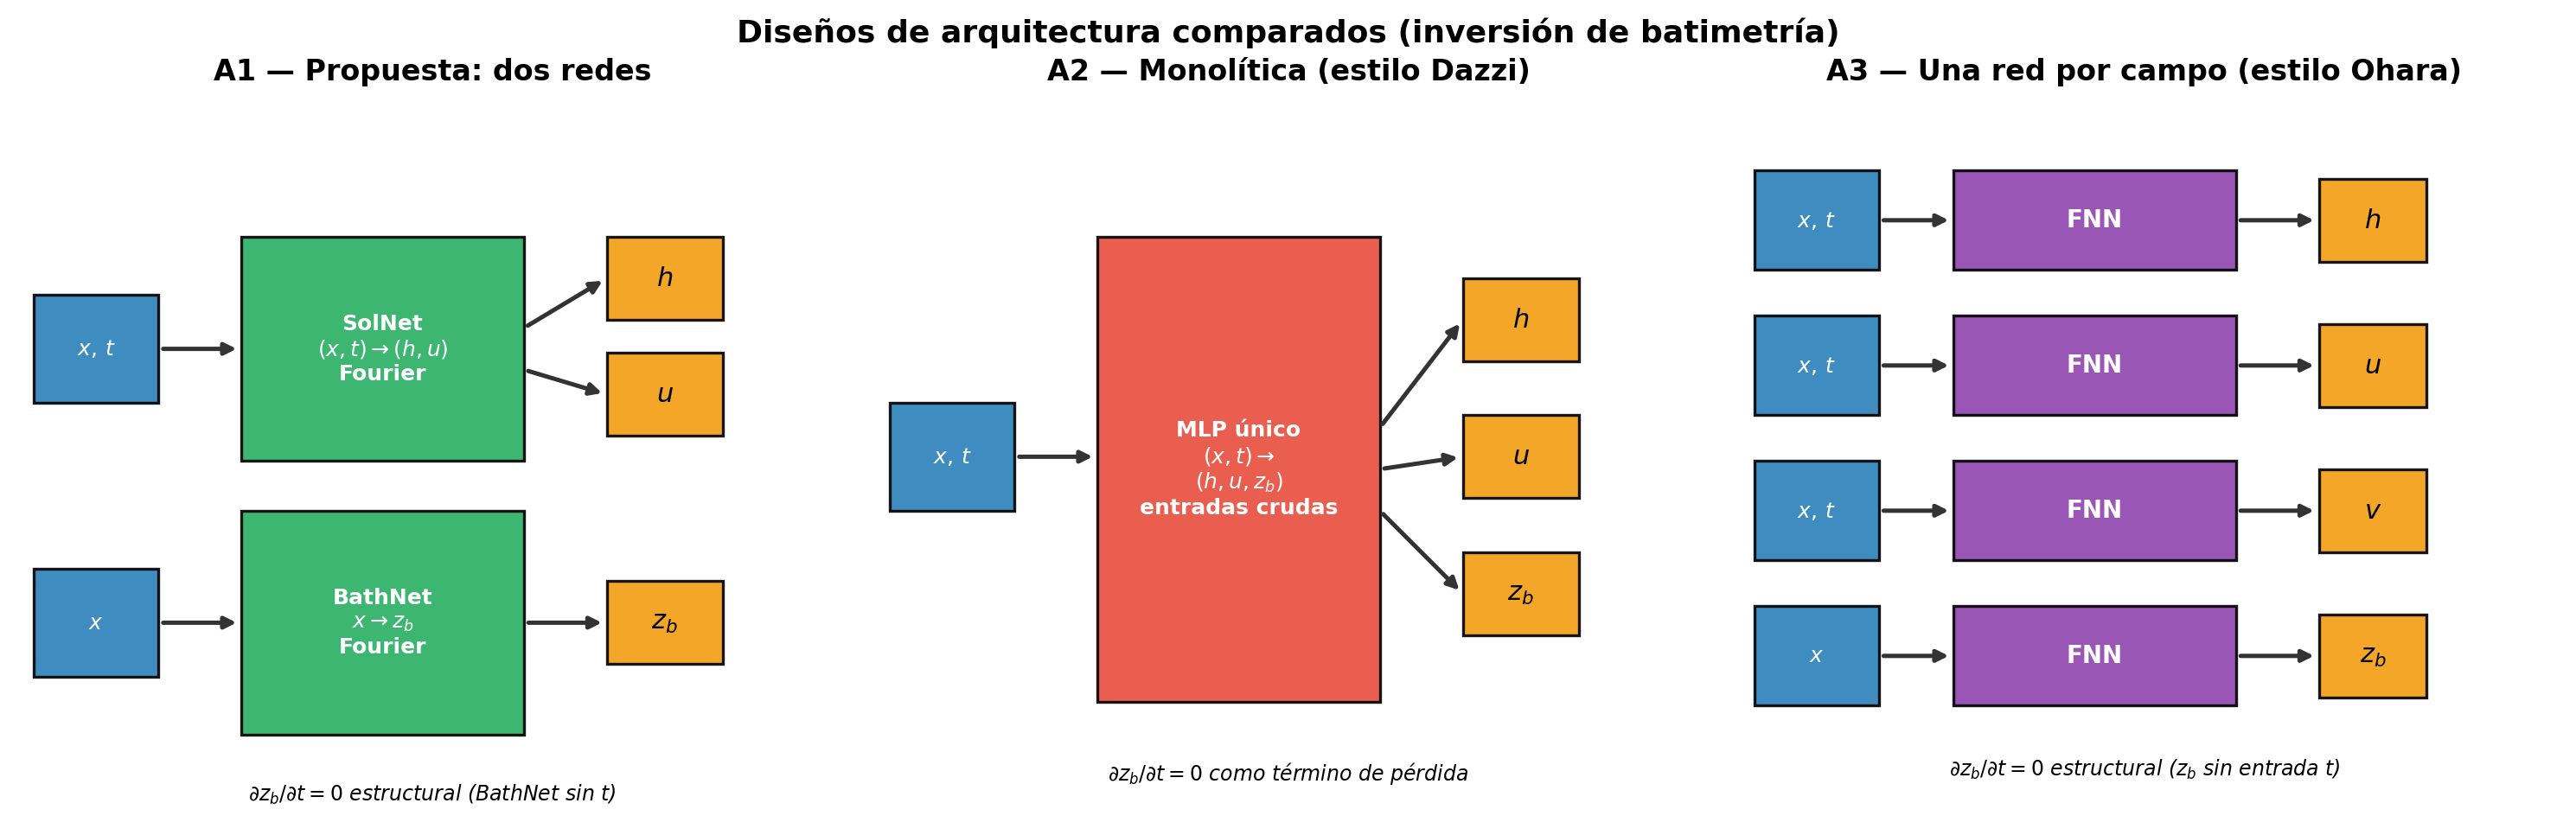
\includegraphics[width=\textwidth]{figures/architecture_designs.png}
  \caption{Los tres diseños de arquitectura comparados, todos para el problema
           inverso de batimetría. \textbf{A1} (propuesta): dos redes ---
           SolNet y BathNet ---, con BathNet sin entrada $t$
           ($\partial\zb/\partial t = 0$ estructural) y embedding de Fourier.
           \textbf{A2} (estilo Dazzi): una red monolítica que produce
           $(h,u,\zb)$ conjuntamente, con $\partial\zb/\partial t = 0$
           impuesto como término de pérdida. \textbf{A3} (estilo Ohara): una
           red totalmente conectada por cada campo de salida. Cada diseño se
           evalúa en el estudio de escalamiento a presupuestos de
           $\approx$20K, 100K y 500K parámetros.}
  \label{fig:arch}
\end{figure}

\subsection{Caso base}

Las ecuaciones de aguas someras, sus hipótesis de validez y la notación se
introdujeron en la Sección~\ref{sec:problema}. El caso base de este trabajo
(Exp.~1) las especializa a flujo 1D estacionario sin fricción:
%
\begin{align}
  \text{Continuidad:} \quad & \pd{(hu)}{x} = 0 \label{eq:cont} \\
  \text{Momento:}     \quad & u\pd{u}{x} + g\pd{(h + \zb)}{x} = 0 \label{eq:mom}
\end{align}

\subsection{Formas del residuo}

La Sección~\ref{sec:problema} señaló que las SWE admiten formas equivalentes;
su elección es una decisión metodológica y un aporte de este trabajo, evaluado
en la Sección~\ref{sec:ablation}. Se comparan tres formulaciones del residuo,
concretadas para el caso base:

\paragraph{Forma primitiva.}
Residuos directos de \eqref{eq:cont}--\eqref{eq:mom}:
\begin{align}
  r_{\text{cont}} &= u\,\pd{h}{x} + h\,\pd{u}{x}, \label{eq:r-prim-cont}\\
  r_{\text{mom}}  &= u\,\pd{u}{x} + g\Big(\pd{h}{x} + \pd{\zb}{x}\Big).
    \label{eq:r-prim-mom}
\end{align}

\paragraph{Forma primitiva-conservativa.}
Ponderación mediante la matriz $\bm{A}$:
\begin{equation}
  \begin{pmatrix} R_{\text{cont}} \\ R_{\text{mom}} \end{pmatrix}
  = \underbrace{\begin{pmatrix} 1 & 0 \\ u & h \end{pmatrix}}_{\bm{A}}
  \begin{pmatrix} r_{\text{cont}} \\ r_{\text{mom}} \end{pmatrix}
  \label{eq:primcons}
\end{equation}

\paragraph{Forma conservativa.}
Residuos sobre flujos conservativos:
\begin{align}
  R_{\text{masa}} &= \pd{(hu)}{x}, \label{eq:r-cons-masa}\\
  R_{\text{mom}}  &= \pd{}{x}\!\Big(hu^2 + \tfrac{1}{2}gh^2\Big)
                     + gh\,\pd{\zb}{x}. \label{eq:r-cons-mom}
\end{align}

\subsection{Función de pérdida}

\begin{equation}
  \mathcal{L} = \lambda_{\eta}\mathcal{L}_{\eta}
              + \lambda_{\text{PDE}}\mathcal{L}_{\text{PDE}}
              + \lambda_q \mathcal{L}_q
              + \lambda_{\text{BC}}\mathcal{L}_{\text{BC}}
              + \lambda_{\text{TV}}\mathcal{L}_{\text{TV}}
              + \lambda_{\text{Tikh}}\mathcal{L}_{\text{Tikh}}
              + \lambda_{\text{pos}}\mathcal{L}_{\text{pos}}
  \label{eq:loss}
\end{equation}

con (todas las sumas son promedios sobre los puntos correspondientes):
\begin{align*}
  \mathcal{L}_{\eta}       &= \tfrac{1}{|S|}\sum_{i\in S}
                              \big(h_i + z_{b,i} - \eta^{\text{obs}}_i\big)^2, \\
  \mathcal{L}_{\text{PDE}}  &= \tfrac{1}{N_c}\sum_i
                              \big(R_{\text{cont},i}^2 + R_{\text{mom},i}^2\big), \\
  \mathcal{L}_q            &= \tfrac{1}{N}\sum_i (h_i u_i - q)^2, \\
  \mathcal{L}_{\text{BC}}   &= \zb(x_L)^2 + \zb(x_R)^2
                              + \big(h(x_R)-h_{\text{down}}\big)^2, \\
  \mathcal{L}_{\text{TV}}   &= \tfrac{1}{N-1}\sum_i |z_{b,i+1}-z_{b,i}|/\Delta x, \\
  \mathcal{L}_{\text{Tikh}} &= \tfrac{1}{N}\sum_i z_{b,i}^2, \\
  \mathcal{L}_{\text{pos}}  &= \tfrac{1}{N}\sum_i \max(0,-h_i)^2 .
\end{align*}
$\mathcal{L}_\eta$ es la pérdida de datos sobre la superficie libre, evaluada
solo en el subconjunto observado $S$ (admite observaciones dispersas);
$\mathcal{L}_{\text{PDE}}$ el residuo físico de la forma elegida;
$\mathcal{L}_q$ fija el caudal por unidad de ancho conocido $q = hu$;
$\mathcal{L}_{\text{BC}}$ impone fondo nulo en los extremos y la profundidad
prescrita aguas abajo; $\mathcal{L}_{\text{TV}}$ y $\mathcal{L}_{\text{Tikh}}$
regularizan $\zb$ (variación total y Tikhonov); y $\mathcal{L}_{\text{pos}}$
penaliza profundidades negativas. Cuando hay observaciones de velocidad se
añade un término análogo $\mathcal{L}_u = \tfrac{1}{|S|}\sum_{i\in S}
(u_i-u^{\text{obs}}_i)^2$ (peso $\lambda_u$); el Exp.~1 lo explota para
cuantificar el aporte de la velocidad. La Tabla~\ref{tab:pesos} lista los
pesos del caso base. Esta misma función de pérdida, con los mismos pesos, se
emplea para las tres arquitecturas evaluadas (Sección~\ref{sec:protocolo}), de
modo que la comparación aísla el efecto de la arquitectura.

\begin{table}[H]
\centering
\caption{Pesos de pérdida del caso base (Exp.~1).}
\label{tab:pesos}
\begin{tabular}{lc}
\toprule
Término & Peso \\
\midrule
$\lambda_{\eta}$ (datos $\eta$)         & 10 \\
$\lambda_{u}$ (datos $u$, opcional)     & 1 \\
$\lambda_{\text{PDE}}$ (residuo SWE)    & 1 \\
$\lambda_{q}$ (caudal)                  & 10 \\
$\lambda_{\text{BC}}$ (bordes)          & 100 \\
$\lambda_{\text{TV}}$ (variación total) & $10^{-4}$ \\
$\lambda_{\text{Tikh}}$ (Tikhonov)      & $10^{-5}$ \\
$\lambda_{\text{pos}}$ (positividad)    & 10 \\
\bottomrule
\end{tabular}
\end{table}

\subsection{Métricas de evaluación}

La calidad de la batimetría recuperada se cuantifica con:
\begin{align*}
  \RMSE  &= \sqrt{\tfrac{1}{N}\sum_i (\hat z_{b,i}-z_{b,i})^2}, \qquad
  \NRMSE  = \frac{\RMSE}{\max_i z_{b,i} - \min_i z_{b,i}}, \\
  R^2    &= 1 - \frac{\sum_i (\hat z_{b,i}-z_{b,i})^2}
                     {\sum_i (z_{b,i}-\bar z_b)^2}.
\end{align*}
El $\NRMSE$ normaliza por el rango de $\zb$ (convención de Angel et al.\, para
comparar con su $\approx$14--16\,\%); $R^2$ mide la fracción de varianza
explicada.

\subsection{Entrenamiento}

Dos fases: 12K épocas de Adam (lr $= 10^{-3}$, decay $\times 0.5$ cada 2K)
seguidas de 600 pasos de L-BFGS con line search de Wolfe. La segunda fase
proporciona convergencia de segundo orden para el refinamiento final. En el
caso base 1D, el residuo físico se evalúa sobre la malla espacial completa
(puntos de colocación); las observaciones pueden ser un subconjunto disperso
$S$ de esa malla, lo que conecta con el estudio de densidad de observaciones
del Exp.~1 (Sección~\ref{sec:exp}).

\subsection{Protocolo de comparación justa}
\label{sec:protocolo}

Para que las diferencias observadas sean atribuibles al diseño de la
arquitectura y no a factores de confusión, los tres diseños de la
Sección~\ref{sec:arquitecturas} se entrenan bajo un protocolo idéntico:

\begin{itemize}
  \item \textbf{Mismo presupuesto de parámetros.} En cada punto de comparación
        los tres diseños se instancian al mismo presupuesto (pequeño, medio o
        grande); el número de parámetros es el eje que se barre, no una
        variable libre.
  \item \textbf{Mismos datos.} El mismo ground truth y las mismas
        observaciones ($\eta$, o $\eta$ y $u$) en cada caso de prueba.
  \item \textbf{Misma pérdida.} La función de pérdida
        (Ecuación~\ref{eq:loss}), con los mismos pesos.
  \item \textbf{Misma forma del residuo.} La forma primitiva; la ablación de
        la Sección~\ref{sec:ablation} evalúa cuál de las tres formas resulta
        más adecuada.
  \item \textbf{Mismo presupuesto de entrenamiento.} 12K épocas de Adam $+$
        600 pasos de L-BFGS.
  \item \textbf{Mismas semillas.} Tres semillas aleatorias por configuración;
        se reporta media $\pm$ desviación estándar.
  \item \textbf{Mismo hardware.} GPU NVIDIA RTX 4090.
\end{itemize}

\paragraph{Métricas de costo.}
Junto con la precisión ($\RMSE$, $\NRMSE$ y $R^2$ de $\zb$), se reporta el
\emph{costo} de cada configuración:
\begin{itemize}
  \item \textbf{Parámetros entrenables}: el costo de capacidad; es el eje que
        se barre en el estudio de escalamiento (presupuestos pequeño, medio y
        grande).
  \item \textbf{Tiempo de entrenamiento} (wall-time) bajo el presupuesto de
        entrenamiento fijo.
  \item \textbf{Memoria de GPU} (VRAM pico).
\end{itemize}
La comparación contrasta precisión frente a costo: a presupuesto de parámetros
igualado, qué diseño es más preciso; y, a lo largo del barrido, qué diseño
domina la curva precisión-vs-parámetros. El estudio se ejecuta sobre los casos
de prueba Exp.~1, 2 y 3 (Sección~\ref{sec:exp}); sus resultados se reportan en
la Sección~\ref{sec:arch-comp}.
